\chapter{Die Tests und erreichten Ziele}
\label{cha:Analyse}
Dieses Kapitel beschäftigt sich mit den Tests und den erreichten Zielen des implementierten Vorlagenmanagements. Es gibt zwei Arten von Tests die implementiert wurden
\begin{itemize}
	\item die Tests, die nicht auf eine \emph{CDI}-Umgebung angewiesen sind und 
	\item die Tests, die auf eine \emph{CDI}-Umgebung angewiesen sind.
\end{itemize}

\section{Die Tests}
Dieser Abschnitt beschäftigt sich mit den implementieren Tests des Vorlagenmanagements und der implementierten Konfiguration für die Tests. Für die Tests wurden folgende Bibliotheken verwendet.
\begin{itemize}
	\item\emph{JUnit4}
	\newline
	ist eine Bibliothek, die ein vollwertiges Test-\emph{Framework} ist, mit dem wiederholbare und reproduzierbare Tests implementiert werden können. \emph{JUnit} ist als Standard für Tests in \emph{Java} anzusehen.
	\item\emph{DeltaSpike}
	\newline
	ist ein Projekt von der \emph{Apache-Software-Foundation (ASF)}, die portable \emph{CDI}-Erweiterungen in Form von Bibliotheken bereitstellt und auch eine Bibliothek für \emph{JUnit}-Tests in einer \emph{CDI}-Umgebung, basierend auf der Bibliothek \emph{JUnit}, bereitstellt.
	\item\emph{H2}
	\newline
	ist eine Bibliothek, die eine Bibliothek, die eine \emph{In-Memory}-Datenbank zur Verfügung stellt.  
\end{itemize}
\ \newline
Alle implementierten Tests sind nicht auf einen Anwendungsserver angewiesen und sind in jeder Entwicklungsumgebung wie z.B \emph{Eclipse} oder \emph{Intellij} und bei einem Kompilieren über das \emph{Buildtool Maven} ausführbar.
\newline
\newline
Die Tests wurden wie folgt organisiert.
\begin{itemize}
	\item\emph{com.clevercure.mailing.test.*} 
	\newline
	ist das \emph{Java}-Paket in dem alle implementierten Tests liegen. 
	\item\emph{*.[toTestClass]Tests}
	\newline
	ist das \emph{Java}-Paket, für eine zu testende Klasse, wobei der Paketname den Namen der zu testenden Klasse mit dem Suffix Tests enthält.
	\item\emph{[toTestMethod]Test.java}
	\newline
	ist die implementierte Testklasse für die Tests einer Methode der zu testenden Klasse.
	\item\emph{test\_case}
	\newline
	ist der Name der einzelnen Testmethoden, der wiedergibt, was an einer Methode getestet wird. 
\end{itemize}
\ \newline
Die vorgestellte Konvention der Tests wurde so umgesetzt, sofern es möglich war, da es auch Tests gibt, die nicht mit dieser Konvention definiert werden können.

\subsection{Die Tests der \emph{CDI}-Integration}
Die Tests aus Abbildung \ref{fig:tests-template-cdi} testen die Implementierungen des Artefakts \emph{mailing-moule-template-cdi}, das die \emph{CDI}-Integration des Variablenmanagements enthält. Es werden die Klassen wie
\begin{itemize}
	\item die Klasse \emph{TemplateCdiExtension},
	\item die Klasse \emph{VariableResolverFactoryProvider},
	\item die Klasse \emph{CdiTemplateUtils} und 
	\item die Klasse \emph{TemplateResourceProducer} getestet.
\end{itemize}
\ \newline
Diese Tests sind nur lauffähig in einer \emph{CDI}-Umgebung, die mit \emph{DeltaSpike} im Klassenpfad gestartet werden kann. Im Klassenpfad der Tests wurden Variablen und eine Implementierung der Klasse \emph{VariableResolverFactory} implementiert. Mit diesen Tests wird sichergestellt, dass die \emph{CDI}-Integration des Vorlagenmanagements, aus Sicht der Implementierung, korrekt funktioniert. Diese Tests gewährleisten nicht, dass die \emph{CDI}-Integration in jeder Implementierung einer \emph{CDI}-Umgebung funktioniert, da es hier durchaus Unterschiede geben kann. Um garantieren zu können, dass das Vorlagenmanagement in der verwendeten implementierten \emph{CDI}-Umgebung funktioniert, müssten Integrationstests implementiert werden, die im verwendeten Anwendungsserver ausgeführt werden. Trotzdem gewährleisten die implementierten Tests, dass die \emph{CDI}-Integration korrekt funktioniert, da die Wahrscheinlichkeit, dass es zu Problemen kommt,  äußert gering ist.
\newpage

\begin{figure}[h]
\centering
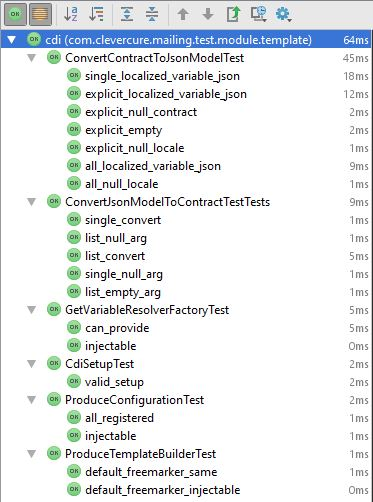
\includegraphics[scale=0.9]{tests-template-cdi}
\caption{Die Tests des Artefakts \emph{mailing-moule-template-cdi}}
\label{fig:tests-template-cdi}
\end{figure}

\subsection{Die Tests der \emph{JSF}-Integration}
Die Tests aus Abbildung \ref{fig:tests-template-jsf} testen die Implementierungen des Artefakts \emph{mailing-module-template-jsf}, das die \emph{JSF}-Integration des Variablenmanagements enthält. Es wird der implementierte \emph{FacesConverter FreemarkerTemplateConverter} getestet. Obwohl die Klasse \emph{FreemarkerTemplateConverter} innerhalb des \emph{JSF´-Framworks} verwendet wird, ist es nicht notwendig eine \emph{JSF}-Umgebung zu simulieren oder zu starten. Der Konverter greift nicht auf die Formalparameter \emph{UIComponent} und \emph{FacesContext} zu, daher ist es nicht notwendig \emph{Mocks} für diese Objekte zur Verfügung zu stellen.
\newline
\newline
Diese Tests sind aber auf eine \emph{CDI}-Umgebung angewiesen, da in der Implementierung mit der \emph{CDI}-Erweiterung interagiert wird und \emph{CDI-Beans} verwendet werden.
\newpage

\begin{figure}
\centering
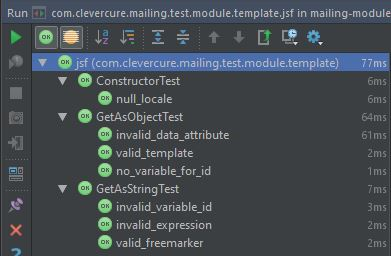
\includegraphics[scale=0.9]{tests-template-jsf}
\caption{Die Tests des Artefakts \emph{mailing-moule-template-jsf}}
\label{fig:tests-template-jsf}
\end{figure}

\subsection{Die Tests des Vorlagenmanagements}
Die Tests aus Abbildung \ref{fig:tests-template-impl} testen die Implementierungen des Artefakts \emph{mailing-module-template-logic-impl}, welches die Implementierungen des Vorlagenmanagements enthält. Es werden die Klassen
\begin{itemize}
	\item \emph{VariableConfigurationImpl} und
	\item \emph{FreemarkerTemplateDataJsonBuilder} getestet.
\end{itemize}
\ \newline
Diese Tests sind nicht abhängig von einer \emph{CDI}-Umgebung und können mit der Bibliothek \emph{JUnit4} alleine getestet werden. Es wird getestet ob Variablen korrekt registriert werden und in einem Objekt der Klasse \emph{VariableConfigurationImpl} korrekt verwaltet werden und ob die Klasse \emph{FreemarkerTemplateDataJsonBuilder} in der Lage ist ein \emph{JSON}-Datenobjekt repräsentiert über ein Objekt der Klasse \emph{TemplateRequestJson} zu produzieren, dass die Daten für eine Voralge hält.
\newline
\newline
Es sollten noch weitere Tests für die beiden Klassen 
\begin{itemize}
	\item\emph{FreemarkerTemplateProcessor} und
	\item\emph{FreemarkerTemplateMetadata} implementiert werden.
\end{itemize}
\ \newline
Die aufgelisteten Klassen werden zwar indirekt über die Tests aus Abbildung \ref{fig:tests-template-impl} getestet, sollten trotzdem auch in eigenen Tests getestet werden.
\newpage

\begin{figure}[h]
\centering
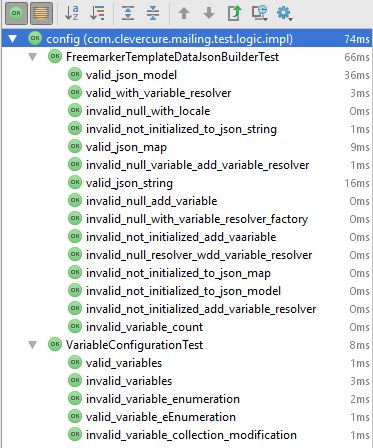
\includegraphics[scale=0.7]{tests-template-impl}
\caption{Die Tests des Artefakts \emph{mailing-moule-template-logic-impl}}
\label{fig:tests-template-impl}
\end{figure}

\section{Die erreichten Ziele}
Dieser Abschnitt beschäftigt sich mit den erreichten Ziele des implementierten Vorlagenmanagements, dessen Integrationen in eine \emph{CDI}-Umgebung und \emph{JSF}, sowie der implementierten Beispielwebanwendung. Es wurden alle Anforderung, die im Kapitel \ref{cha:Zielsetzung} vorgegeben wurden, erfüllt. Der nächste Schritt ist die Integration des Vorlagenmanagements in die Anwendungen
\begin{itemize}
	\item\emph{CleverWeb},
	\item\emph{CleverSupport} und
	\item\emph{CleverInterface}.
\end{itemize}
\ \newline
Die Integration in die Anwendung \emph{CleverInterface} wird warten müssen, bis die verwendete Laufzeitumgebung \emph{IIB Java 8} unterstützt. Sollte \emph{IIB Java 8} nicht in absehbarer Zeit unterstützen, so wird man das Vorlagenmanagement auf \emph{Java 7} migrieren müssen, was aber nicht anzuraten ist. Die Beispielwebanwendung hat aufgezeigt, wie einfach es ist eine \emph{JSF}-Seite für die Verwaltung von Vorlagen zu implementieren und wie einfach \emph{E-Mails} über eine Geschäftslogik erstellt werden können. Somit sollten sich die Integrationen in die Anwendungen \emph{CleverWeb} und \emph{CleverSupport} einfach und schnell realisieren lassen. 

\subsection{Das \emph{CKEditor-Plugin} für das Vorlagenmanagement}
Es wurde erfolgreich ein \emph{Plugin} für den \emph{CKEditor} implementiert, sowie ein Variablenmanagement für die \emph{Browser}-seitige Verwaltung der Variablen. Wie in Abschnitt \ref{sec:sub-typescript-javascript} vorgegeben, wurde das \emph{CKEditor-Plugin} und das Variablenmanagement in \emph{TypeScript} implementiert. Das \emph{CKEditor-Plugin} und das Variablenmanagement wurden getrennt voneinander in eigenen Quelltextdateien implementiert. Die implementierten \emph{TypeScript}-Quelltexte befinden sich zurzeit noch in der Beispielwebanwendung, da die Entwicklung in einem eigenen Projekt nicht möglich war, da das \emph{Hot-Code-Deployment} für \emph{Java}-Ressourcen (src/main/resources) nicht unterstützt wird. Diese Quelltextdateien können einfach in ein anderes Projekt verschoben werden. Die Quelltextdateien werden jetzt noch über die Entwicklungsumgebung kompiliert. In Zukunft können die \emph{TypeScript}-Quelltextdateien über das \emph{Maven-Build-Plugin maven-grunt-plugin} auch automatisiert bei jedem \emph{Maven-Build} kompiliert werden, was sehr zu empfählen ist.

\subsection{Die \emph{CDI}-Integration des Vorlagenmanagements}
Es wurde erfolgreich die Integration des Vorlagenmanagement in eine \emph{CDI}-Umgebung implementiert. Die in Abschnitt \ref{sec:sub-impl-integartion-cdi} behandelte Integration in eine \emph{CDI}-Umgebung, wurde über eine portierbare \emph{CDI}-Erweiterung realisiert. Als nächster Schritt könnten auch Variablen unterstützt werden, die nicht über eine \emph{Enum} definiert werden. Dazu müsste die Methode \emph{processCdiVariableContracts}  der implementierte Klasse \emph{TemplateCdiExtension} und die Klasse \emph{VariableConfigurationImpl} erweitert werden. Die Klasse \emph{TemplateCdiExtension} müsste die registrierten Type der Schnittstelle \emph{VariableContract} in einem Behälter verwalten und die Klasse \emph{VariableConfigurationImpl} müsste in der Lage sein, die registrierten Variablen dynamisch aus einer \emph{CDI}-Umgebung zu holen. Es müsste eine Schnittstelle eingeführt werden, die das Holen der Variablen aus der \emph{CDI}-Umgebung für die Klasse \emph{VariableConfigurationImpl} abstrahiert, damit keine Abhängigkeiten zu Klassen von \emph{CDI} verwendet werden müssen.

\subsection{Das Vorlagenmanagement in \emph{JSF}}
Es wurde erfolgreich eine Integration in \emph{JSF} implementiert, wobei diese Integration über den implementierten \emph{FacesConverter} \emph{FreemarkerTemplateConverter} erreicht wurde, der die Vorlagen von ihrer \emph{HTML}-Repräsentation in die \emph{Freemarker}-Repräsentation konvertieren kann. Wie in Abschnitt \ref{sec:sub-impl-integartion-jsf} vorgestellt, wurde die gemeinsame Logik in einer abstrakte Klasse \emph{AbstractTemplateConverter} gekapselt, der nur bekanntgegeben werden muss, welche konkrete Implementierung, definiert über ein Annotationsliteral für den Qualifizierer, genutzt werden soll. Wenn man auf \emph{JSF 2.3} wechselt, könnte man die dynamische Interaktion mit der \emph{CDI}-Umgebung durch statische Injektionspunkte ersetzten, die auch beim Start der \emph{CDI}-Umgebung validiert werden. 

\subsection{Das Vorlagenmanagement in \emph{Mail}-DB-Schema}
Die Integration der Vorlagen in des \emph{Mail-DB}-Schema war die die einfachste Aufgabe, da hier lediglich eine einfache Datenstruktur definiert werden muss, die in der Lage ist, die Vorlagen mehrsprachig persistent zu halten. Prinzipiell ist eine Vorlage auf einer Datenbank als Zeichenkette präsent, wobei nur auf die Größe der Zeichenkette geachtet werden muss. Sollte das Vorlagenmanagement auch in anderen Bereichen verwendet werden, so könnte man eine eigene Datenstruktur definieren, die über \emph{JPA}-Entitäten abgebildet werden könnte und in den verschiedenen Datenbanken verwendet werden könnte.
